\documentclass[12pt]{article}
\usepackage{amsmath,amssymb,amsthm, amsfonts,tcolorbox}
\usepackage{graphicx,color}
\usepackage{color}
\usepackage{tikz,pgfplots}
\usetikzlibrary{decorations.pathreplacing,calligraphy}
\usetikzlibrary{shapes.geometric}
\usetikzlibrary{shapes.multipart}
\usetikzlibrary{arrows}
\usetikzlibrary{calc}
\usetikzlibrary{arrows.meta}
\usetikzlibrary{arrows}
\usetikzlibrary{patterns}
\usetikzlibrary{shapes,snakes}
\usetikzlibrary{decorations.markings}
\tikzset{vtx/.style={inner sep=1.7pt, outer sep=0pt, circle,fill,draw}, % style of a vertex
vtx red/.style={inner sep=2.7pt, outer sep=0pt, circle, fill=red,draw}, 
vtx blue/.style={inner sep=2.7pt, outer sep=0pt, circle, fill=blue,draw}, 
vtx green/.style={inner sep=2.7pt, outer sep=0pt, circle, fill=black!30!green,draw}, 
vtx gray/.style={inner sep=2.7pt, outer sep=0pt, circle, fill=gray!30!white,draw}, 
vtx3/.style={inner sep=1.2pt, outer sep=0pt, regular polygon, regular polygon sides=3, draw},
vtx4/.style={inner sep=1.7pt, outer sep=0pt, regular polygon, regular polygon sides=4, draw},
vtx5/.style={inner sep=1.7pt, outer sep=0pt, regular polygon, regular polygon sides=5, draw},
vtx_box/.style={inner sep=2pt, outer sep=0pt, rectangle, draw, fill=white},
blueish/.style={color=blue},
reddish/.style={color=red},
greenish/.style={color=black!30!green},
edge_blueish/.style={color=blue,line width=2pt},
edge_reddish/.style={color=red,line width=2pt,dashed},
edge_greenish/.style={color=black!30!green,line width=2pt, densely dotted},
edge_orange/.style={color=orange,line width=2pt},
directed edge/.style={decoration={markings, mark=at position 0.5 with {\arrow{Latex}}},  postaction={decorate}},
}

\begin{document}

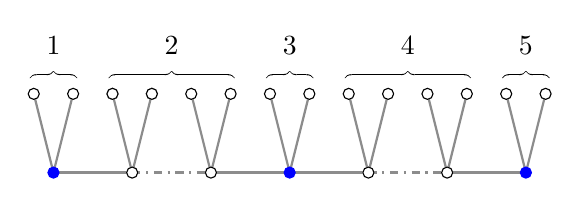
\begin{tikzpicture}
        \draw[thick, gray!90]    (0,0) -- (1,0);
        \draw[thick, gray!90]    (2,0) -- (3,0);
        \draw[thick, gray!90]    (3,0) -- (4,0);
        \draw[thick, gray!90]    (5,0) -- (6,0);
        \draw[thick, dash dot, gray!90]    (1,0) -- (2,0);
        \draw[thick, dash dot, gray!90]    (4,0) -- (5,0);
        
        \draw[thick, gray!90]    (-.25,1) -- (0,0) -- (.25,1);
        \draw[thick, gray!90]    (.75,1) -- (1,0) -- (1.25,1);
        \draw[thick, gray!90]    (1.75,1) -- (2,0) -- (2.25,1);
        \draw[thick, gray!90]    (2.75,1) -- (3,0) -- (3.25,1);
        \draw[thick, gray!90]    (3.75,1) -- (4,0) -- (4.25,1);
        \draw[thick, gray!90]    (4.75,1) -- (5,0) -- (5.25,1);
        \draw[thick, gray!90]    (5.75,1) -- (6,0) -- (6.25,1);
        
        \draw [decorate, decoration = {calligraphic brace}] (-.3,1.2) --  (.3,1.2);
        \draw [decorate, decoration = {calligraphic brace}] (.7,1.2) --  (2.3,1.2);
        \draw [decorate, decoration = {calligraphic brace}] (2.7,1.2) --  (3.3,1.2);
        \draw [decorate, decoration = {calligraphic brace}] (3.7,1.2) --  (5.3,1.2);
        \draw [decorate, decoration = {calligraphic brace}] (5.7,1.2) --  (6.3,1.2);
        
        \node[circle, label={90:$1$}] at (0,1.2) {};
        \node[circle, label={90:$2$}] at (1.5,1.2) {};
        \node[circle, label={90:$3$}] at (3,1.2) {};
        \node[circle, label={90:$4$}] at (4.5,1.2) {};
        \node[circle, label={90:$5$}] at (6,1.2) {};
        

        
        
        \filldraw[blue] (0,0) circle (2pt);
        \filldraw[white] (1,0) circle (2pt);
        \draw[black] (1,0) circle (2pt);
        \filldraw[white] (2,0) circle (2pt);
        \draw[black] (2,0) circle (2pt);
        \filldraw[blue] (3,0) circle (2pt);
        \filldraw[white] (4,0) circle (2pt);
        \draw[black] (4,0) circle (2pt);
        \filldraw[white] (5,0) circle (2pt);
        \draw[black] (5,0) circle (2pt);
        \filldraw[blue] (6,0) circle (2pt);
        
        \filldraw[white] (-.25,1) circle (2pt);
        \draw[black] (-.25,1) circle (2pt);
        \filldraw[white] (.25,1) circle (2pt);
        \draw[black] (.25,1) circle (2pt);
        
        \filldraw[white] (.75,1) circle (2pt);
        \draw[black] (.75,1) circle (2pt);
        \filldraw[white] (1.25,1) circle (2pt);
        \draw[black] (1.25,1) circle (2pt);
        
        \filldraw[white] (.75,1) circle (2pt);
        \draw[black] (.75,1) circle (2pt);
        \filldraw[white] (1.25,1) circle (2pt);
        \draw[black] (1.25,1) circle (2pt);
        
        \filldraw[white] (1.75,1) circle (2pt);
        \draw[black] (1.75,1) circle (2pt);
        \filldraw[white] (2.25,1) circle (2pt);
        \draw[black] (2.25,1) circle (2pt);
        
        \filldraw[white] (2.75,1) circle (2pt);
        \draw[black] (2.75,1) circle (2pt);
        \filldraw[white] (3.25,1) circle (2pt);
        \draw[black] (3.25,1) circle (2pt);
        
        \filldraw[white] (3.75,1) circle (2pt);
        \draw[black] (3.75,1) circle (2pt);
        \filldraw[white] (4.25,1) circle (2pt);
        \draw[black] (4.25,1) circle (2pt);
        
        \filldraw[white] (4.75,1) circle (2pt);
        \draw[black] (4.75,1) circle (2pt);
        \filldraw[white] (5.25,1) circle (2pt);
        \draw[black] (5.25,1) circle (2pt);
        
        \filldraw[white] (5.75,1) circle (2pt);
        \draw[black] (5.75,1) circle (2pt);
        \filldraw[white] (6.25,1) circle (2pt);
        \draw[black] (6.25,1) circle (2pt);
        
        
        
        
        \end{tikzpicture}

\end{document}